\chapter*{Estrazione Automatica di Informazione Simbolica Da Immagini}
\addcontentsline{toc}{chapter}{Estrazione Automatica di Informazione Simbolica Da Immagini}
	
	\section*{Introduzione}
	\addcontentsline{toc}{section}{Introduzione}
	Questo documento descrive i principali passi dello sviluppo di un modulo software di computer vision che effettua l'analisi di immagini e comunica i risultati all'architettura cognitiva \mbox{\emph{ACT-R}}\footnote{ACT-R è un'architettura cognitiva, cioè un framework che modella la struttura e il comportamento umano. Per maggiori informazioni, vedere~\url{act-r.psy.cmu.edu}.}.
	In particolare, il programma ha il compito di riuscire a riconoscere le forme geometriche contenute nelle immagini, i loro colori ed effettuare valutazioni qualitative e quantitative su tali oggetti.

	L'attività è stata svolta presso il \emph{Center for Cognitive Science} dell'università \emph{Albert-Ludwigs-Universität Freiburg} della città di Friburgo.
	Le attività di ricerca del centro, che come suggerisce il nome hanno come ambito principale le \emph{scienze cognitive}\footnote{\emph{Le scienze cognitive sono un gruppo di discipline che hanno come scopo lo studio delle capacità cognitive delle menti naturali o artificiali, della possibilità di trasmettere questo sapere agli altri e di averne consapevolezza. La scienza cognitiva è la specifica materia, tra le scienze cognitive, che spiega i modi in cui menti naturali o artificiali filtrano e colgono informazioni percettive, le rielaborano e riescono a intraprendere delle decisioni in base alle circostanze esperite, tanto da "reagire" al mondo esterno anche elaborando degli artefatti}~\cite{legrenzi2005prima}.}, 	
	al momento si focalizzano sul ragionamento spaziale\footnote{Il ragionamento spaziale è una disciplina che si occupa del ragionamento basato sugli oggetti nello spazio; in particolare studia le astrazioni dei concetti spaziali della conoscenza di base sulla quale si basa la prospettiva umana della realtà fisica.} e i ricercatori utilizzano ACT-R come strumento di supporto per i loro studi. 
	
	In questo contesto, il lavoro discusso in questo documento rappresenta una parte del lavoro sviluppato da un team di tre persone, il cui obiettivo finale risulta essere quello di migliorare la percezione dell'architettura cognitiva, rendendola più simile a quella umana.  
	Una delle maggiori limitazioni di \mbox{ACT-R}, infatti, è il fatto che essa lavora in un ambiente virtuale troppo semplice per rappresentare la realtà. 
	Il software sviluppato rappresenta un punto di partenza per permettere ad \mbox{ACT-R} di elaborare oggetti direttamente dal mondo reale, superando tale limite.
	 
	Dal momento che allo stato attuale l'architettura cognitiva non presenta dei moduli propri per l'elaborazione dei dati visuali, il software sviluppato è stato creato esternamente come software indipendente. 
	Ciò ha permesso di utilizzare la libreria esterna \mbox{\emph{OpenCV}} per l'elaborazione di immagini e richiede l'introduzione di un protocollo di comunicazione client-server in modo da rendere possibile la comunicazione tra \mbox{ACT-R} e il modulo di visione sviluppato.

	\section*{L'ambiente di lavoro}
	\addcontentsline{toc}{section}{L'ambiente di lavoro}
	L'attività è stata condotta presso il \emph{Center for Cognitive Science} dell'università \emph{Albert-Ludwigs-Universität Freiburg} della città di Friburgo in Germania. Tale centro ricerca nell'ambito delle \emph{scienze cognitive}, in particolare studia il \emph{ragionamento spaziale}.

	Le scienze cognitive sono delle discipline che studiano le capacità cognitive della mente, indipendentemente dalla sua natura artificiale o naturale, e spiegano le modalità con cui essa raccoglie e filtra le informazioni percettive ricevute, le rielabora e, sulla base della conoscenza ottenuta, prende delle decisioni che causano poi le reazioni dell'agente agli eventi del mondo esterno. 
	Ciò che viene studiato, in particolare, sono le modalità con cui pensiero, emozione, immaginazione, intelletto e creatività vengono formati~\cite{legrenzi2005prima}.
	La sfida per queste discipline sta nello studiare questi aspetti data l'impossibilità di osservare i processi cognitivi umani nelle diverse fasi in cui si sviluppano. 
	
	Un aspetto caratterizzante di tutte le scienze cognitive è la loro natura multidisciplinare: esse infatti accorpano informazioni provenienti da discipline eterogenee (fisiologia, neurologia, intelligenza artificiale, filosofia e psicologia) al fine di creare un modello per la mente che sia il più generale possibile~\cite{legrenzi2005prima}. 

	La cognizione spaziale è la scienza cognitiva che studia acquisizione, organizzazione, utilizzo e revisione della conoscenza riguardante gli ambienti spaziali~\cite{r8Cspace}. L'ambito di applicabilità di tale disciplina è molto vasto e comprende sia ambienti reali che modelli astratti e prevede agenti sia umani che automatici.
	Fondamentale per questa materia è lo studio del processo di ragionamento, che comprende la successione di eventi che portano alla formazione di conoscenza a partire da una serie di premesse. 
	
	Una delle grandi sfide che il centro di ricerca si pone è quella di \emph{gettare le basi per nuove teorie cognitive, riguardanti il ragionamento e la pianificazione, applicando metodi di intelligenza artificiale ed esperimenti comportamentali}.

 

	\section*{Lo stato dell'arte}
	\addcontentsline{toc}{section}{Lo stato dell'arte}
	Di seguito si descrivono i due principali strumenti utilizzati per questo progetto: la libreria di computer vision \emph{\mbox{OpenCV}} e l'architettura cognitiva \mbox{\emph{ACT-R}}.
		
			\subsection*{ACT-R}
			\addcontentsline{toc}{subsection}{ACT-R}
				\mbox{ACT-R} è un'\emph{architettura cognitiva}, cioè l'implementazione di una teoria riguardante il sistema cognitivo umano. Come tale, esso modella struttura e comportamento del cervello umano cercando di spiegare come le diverse componenti collaborano tra loro e formano la mente umana.
				
				La teoria di \mbox{ACT-R} si basa sulla \emph{teoria unificata della cognizione} (Unified theory about cognition), sviluppata da John Robert Anderson, docente presso la Carnegie Mellon University. Il concetto fondamentale di tale teoria è che la mente umana, che è separata in diversi moduli indipendenti, ognuno dotato delle proprie funzioni, nel momento di effettuare un comportamento, agisca come un sistema integrato in cui ciascun componente svolge una precisa funzione e può comunicare con gli altri grazie a specifiche connessioni~\cite{Anderson04anintegrated}.

				Un altro pilastro fondamentale su cui si basa la teoria di \mbox{ACT-R} è la distinzione tra \emph{memoria dichiarativa} e \emph{memoria procedurale}. La prima rappresenta fatti e nozioni che l'essere umano sa ed è conscio di sapere. Per richiamare questo tipo di conoscenza, l'essere umano deve effettuare un processo consapevole. La seconda, invece, si riferisce a tutte quelle abilità e capacità che l'essere umano sa ma che ha imparato in maniera implicita. Esempi di questo tipo di conoscenza sono la lettura e la scrittura~\cite{anderson1976language}. 

				Gli elementi di base dell'architettura di \mbox{ACT-R} sono \emph{chunk} e \emph{produzioni}.
				I chunk rappresentano la memoria dichiarativa e sono delle strutture dati caratterizzate da un tipo, chiamato \emph{type}, e da una lista di coppie, ognuna delle quali è costituita da un attributo, chiamato \emph{slot}, e da un valore, chiamato \emph{value}.
				Le produzioni possono essere paragonate a funzioni e definiscono la sequenza di azioni che possono essere effettuate.
				Ogni produzione presenta un insieme di precondizioni che determinano le condizioni che devono essere verificate affinchè la funzione possa essere eseguita ~\cite{actr6refman}.

				Dal punto di vista dell'architettura, \mbox{ACT-R} è organizzato in \emph{moduli}.
				Ciascun modulo è costituito da chunk e da produzioni e svolge un insieme determinato di funzioni cognitive. 
				Essi sono l'analogo dei gruppi di neuroni che si attivano nel cervello nel momento in cui viene effettuata una determinata azione da parte dell'essere umano.
				I moduli sono indipendenti ma possono comunicare tra loro tramite dei \emph{buffer}. 
				La comunicazione, che essenzialmente è uno scambio di chunk, avviene necessariamente in maniera seriale, mentre le operazioni dei diversi moduli possono avvenire in parallelo ~\cite{actr6refman}.
				
				\mbox{ACT-R} è in grado di effettuare infiniti ragionamenti, indipendentemente dal compito da eseguire. 
				Per essere in grado di eseguire una singola attività, tuttavia, necessita di uno specifico \emph{modello}.
				Ciascun modello contiene le assunzioni di chi scrive il modello riguardo al determinato compito da eseguire.
				Tali assunzioni sono espresse sottoforma di produzioni e interagiscono con i moduli durante l'esecuzione, atto che produce una serie di operazioni atomiche cognitive che passo dopo passo portano alla soluzione del compito~\cite{Sears2012}. 
				
				Le operazioni presentano delle misure qualitative e quantitative sulla qualità dell'azione stessa, come la correttezza della soluzione trovata e il tempo necessario per completare l'operazione. 
				Ciò conferisce ai modelli la possibilità di predire la sequenza delle azioni cognitive prodotte dagli esseri umani quando provano a risolvere lo stesso compito. 
				Effettuare dei confronti con le prestazioni degli esseri umani permette di misurare la qualità del modello~\cite{Sears2012}.

				Dal punto di vista informatico, \mbox{ACT-R} è scritto in lisp e fornisce una sintassi specifica, simile al lisp, per scrivere i modelli.

			\subsection*{OpenCV}
			\addcontentsline{toc}{subsection}{OpenCV}
				%intro
				\mbox{OpenCV}, acronimo di Open Computer Vision, è una libreria per la computer vision, sviluppata inizialmente da Intel e supportata poi dall'incubatore tecnologico Willow Garage.
				La libreria è multipiattaforma ed è rilasciata sotto una licenza BSD che la rende gratuita ed open source. 
				È stata sviluppata per supportare applicazioni in tempo reale e perciò è caratterizzata da una grande efficienza computazionale.
				La versione 2.4 contiene più di 2500 algoritmi che coprono molte aree della computer vision.

				% computer vision
				La computer vision è essenzialmente la trasformazione di un'immagine o di un video in una nuova rappresentazione che può essere anche di natura completamente differente rispetto al dato iniziale. 
				L'obiettivo potrebbe essere, ad esempio, una versione in scala di grigi dell'immagine originale, oppure si potrebbe desiderare che il calcolatore sia in grado di prendere una decisione a partire dalle informazioni estratte dall'immagine in ingresso.
				In entrambi i casi si sta parlando di computer vision~\cite{bradski2008learning}.
		
				In generale, la complessità di operazioni di questo tipo risulta essere molto elevata. 
				Ciò che per un essere umano viene percepito come un'attività molto semplice, infatti, può risultare un'operazione molto complessa per un calcolatore.
				Quest'ultimo rappresenta l'immagine tramite matrice di numeri. 
				Tale rappresentazione rende complesse molte delle operazioni di visione, comprese quelle più semplici come, per esempio, il riconoscimento di un semplice oggetto.
				Purtroppo al momento questa modalità di descrizione è la migliore alternativa tra le possibilità esistenti~\cite{bradski2008learning}.

				Oltre alla rappresentazione matriciale, uno dei motivi che rendono così complicata la computer vision è la necessità molto frequente di ricostruire un mondo tridimensionale a partire da un'immagine bidimensionale. 
				Questo è un problema mal posto. 
				Diretta conseguenza di ciò è l'esistenza di infinite soluzioni, cioè infinite ricostruzioni tridimensionali del mondo a partire dall'immagine bidimensionale.
				In particolare, la soluzione dipende dall'angolo con cui si analizza l'immagine~\cite{bradski2008learning}.

				Un fattore che aumenta ulteriormente la complessità dei compiti è la presenza del rumore, che raggruppa tutte le possibili cause di variabilità presenti nel mondo: tempo atmosferico, luminosità, riflessi, movimenti, deformazioni dovute alle lenti o ai sensori e altri fenomeni.
				Il rumore può essere classificato in noto a priori, quindi prevedibile, e non noto a priori, quindi non prevedibile. 
				Il primo, essendo conosciuto, può essere corretto a tal punto da essere completamente eliminato.
				È questo, ad esempio, il caso della deformazione delle lenti delle videocamere.
				Il secondo, invece, essendo casuale, non può essere del tutto eliminato ma può essere solamente ridotto.
				Tipicamente si utilizzano metodi statistici per gestire questo secondo tipo di rumore~\cite{bradski2008learning}. 
			 
				Un metodo per facilitare le operazioni di computer vision è introdurre dell'informazione contestuale. 
				In particolare, più il problema è vincolato, più è facile utilizzare i vincoli per semplificare il problema, più la soluzione ottenuta è affidabile.
				In questo modo ovviamente la soluzione perde di generalità e diventa specifica per il problema.
				Le tecniche di machine learning, che estraggono automaticamente l'informazione contestuale e la utilizzano per risolvere i problemi, possono essere sfruttate nelle operazioni di computer vision~\cite{bradski2008learning}.
				
				Storicamente, il progetto OpenCV viene avviato nel 1999 da Intel Research, divisione del gruppo Intel dedicata alla ricerca. 
				L'iniziativa è finalizzata a migliorare le applicazioni che richiedono un alto carico di lavoro della CPU, in particolare quelle legate alla visione artificiale. 
				Le intenzioni iniziali comprendono la creazione di codice ottimizzato per un'infrastruttura standard di base per la visione, la diffusione di essa tra gli sviluppatori, la portabilità e la possibilità di creare sia applicazioni di natura commerciale che gratuite. 
				Nel 2000 viene rilasciata la prima versione alpha, seguita da cinque versioni beta tra il 2001 e il 2005 che portano nel 2006 a \mbox{OpenCV} 1.0.	
				Nel 2008 l'incubatore tecnologico Willow Garage comincia a supportare il progetto e nel 2009 viene rilasciata la versione 2.0. 
				Come stabilito dal nel piano di rilascio, ogni sei mesi viene resa pubblica una nuova versione di \mbox{OpenCV}~\cite{OpenCV:ChangeLogs}.

				La libreria offre numerose funzioni che coprono diversi rami della computer vision.
				In particolare offre strutture dati per la gestione di immagini e video; funzioni per la visualizzazione e per la gestione degli eventi da parte di tastiera e mouse; procedure per l'interazione con il filesystem; possibilità di manipolare le immagini sia tramite matrici che tramite funzioni di algebra vettoriale; supporto alle strutture dati più comuni e funzioni per tutte le operazioni di base di computer vision: filtraggio, riconoscimento di contorni e di angoli, conversione dei colori, campionamento e interpolazione, operazioni morfologiche e istogrammi.
				Inoltre integra molte funzioni per l'analisi strutturale dell'immagine, la calibrazione di telecamere, analisi del movimento, riconoscimento di oggetti e machine learning~\cite{Agam2006}.
				
				Dal punto di vista informatico, la libreria è scritta in C e C++ e presenta interfacce per i linguaggi Python, Java, Ruby e Matlab.
				Dalla versione 2.4 l'architettura è organizzata in moduli, ognuno dei quali svolge specifiche funzioni~\cite{OpenCVDoc}. 
				


	\section*{Gli obiettivi}\label{obiettivi}
	\addcontentsline{toc}{section}{Gli obiettivi}
		%il contesto		
		L'obiettivo ultimo del progetto che comprende questo lavoro è di dotare \mbox{ACT-R} di un sistema visivo che sia il più simile possibile a quello umano.
		Per raggiungere tale intento, i ricercatori sono costantemente alla ricerca di tecniche innovative nel campo della visione artificiale che siano il più possibile di uso generale.
		Tal ricerca, tuttavia, non è facile; infatti, la maggior parte delle pubblicazioni riguardanti la computer vision utilizza informazione contestuale che rende gli algoritmi adatti solamente ai compiti per cui vengono sviluppati.
		
		Questo documento si focalizza solo su un sottoinsieme di funzionalità, cioè quelle che sono state sviluppate dal gruppo di lavoro in cui l'autore di questo documento è stato inserito.	
		Ciò è dovuto al fatto che l'obiettivo dell'intero progetto è molto ambizioso e richiede un tempo ignoto e difficile da stimare a priori. 
		L'autore del documento, invece, è stato inserito per un periodo di tempo limitato in un gruppo di lavoro incaricato di sviluppare soluzioni a problemi specifici, pertanto saranno queste le funzionalità che verranno descritte nei successivi paragrafi.

		%l'obiettivo del team
		L'obiettivo del gruppo di lavoro è quello di creare un software general purpose che riceva in ingresso un flusso video oppure un'immagine ed effettui un processo di riconoscimento di oggetti sui dati in ingresso.
		\mbox{ACT-R} utilizzerà tale software per orientarsi all'interno di un edificio, distinguendo diversi tipi di stanza a partire dagli oggetti riconosciuti all'interno di ciascuna di esse.

		Come funzionalità fondamentale di tale software, il gruppo deve implementare uno strumento per riconoscere forme geometriche nelle immagini di ingresso. 
		Tali forme rappresentano il punto di partenza per effettuare il processo di riconoscimento degli oggetti. 
		Solo le forme riconosciute dallo strumento sviluppato, infatti, verranno poi analizzate più in dettaglio per verificare che rappresentino o meno degli oggetti di interesse.

		%l'obiettivo del software
		Un seconda seconda applicazione dello strumento è di rendere più facile la definizione del modello al creatore di modelli di \mbox{ACT-R}.
		Per capire meglio questo secondo obiettivo è necessario spiegare come un modello viene creato.
		Il creatore di modelli ha bisogno di un insieme di parametri su cui basare le proprie assunzioni riguardanti alle modalità in cui il cervello umano risolve un determinato compito.
		Tali dati vengono raccolti tramite esperimenti, realizzati grazie a strutture e software appositi, in cui alcuni volontari sono chiamati a risolvere diverse istanze dello stesso compito.
		
		Si prenda per esempio l'immagine~\ref{fig:RushHourHumanIta}, che descrive un'istanza del gioco Rush Hour.
		Tale gioco viene utilizzato come test da alcuni psicologi del Centro delle Scienze Cognitive dell'università di Friburgo per confermare alcune loro ipotesi riguardanti i processi cognitivi umani, la cui spiegazione esula da questo documento.
		L'obiettivo del gioco è spostare le automobili colorate al fine di liberare il percorso tra l'auto rossa e l'uscita, che si trova sulla destra del campo di gioco.
		Ogni automobile, rappresentata da un rettangolo, può spostarsi solo in una direzione, cioè quella parallela al lato maggiore di ciascun rettangolo.
		Minore è il numero di spostamenti dell'automobile, migliore è la soluzione. 	

		\begin{figure}[!h]
		  \begin{center} 
			 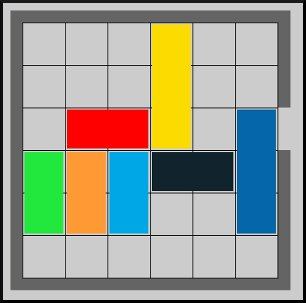
\includegraphics[scale=0.6]{images/ch_03/originale.jpg}	
		  \end{center} 
		  \caption{\textit{Esempio di un istanza del gioco di Rush Hour}}
		  \label{fig:RushHourHumanIta}	
	  	\end{figure}

		Il modello scritto in \mbox{ACT-R} richiede in ingresso la configurazione iniziale di ciascuna delle istanze del problema che si vuole risolvere.
		Al momento, ogni istanza da risolvere, che in \mbox{ACT-R} viene definita tramite una lista di oggetti, deve essere creata manualmente prima della risoluzione. 
		In questo modo, il meccanismo di riconoscimento di \mbox{ACT-R} risulta essere distante da quello umano, il quale riconosce gli oggetti direttamente dall'immagine. 
		Inoltre, dal momento che sia la conferma di un'ipotesi che la stima di determinati parametri richiedono un numero molto alto di istanze, il processo di scrittura manuale comporta una notevole perdita di tempo per i ricercatori.
		Un sistema di riconoscimento automatico, invece, porterebbe una forte innovazione, avvicinando il sistema visuale dell'architettura cognitiva a quello umano, e renderebbe scalabile la creazione di istanze per molti casi di test.
		
		Per ottenere tali obiettivi lo strumento software da sviluppare deve analizzare le immagini che riceve in input; effettuare l'elaborazione, estraendo l'informazione necessaria alla soluzione dei compiti; salvare l'informazione in una struttura dati dedicata e comunicare tutta l'informazione all'architettura cognitiva.
		

	\section*{I Requisiti}
	\addcontentsline{toc}{section}{I Requisiti}	
		Di seguito vengono riportati prima i requisiti funzionali e, successivamente, quelli non funzionali.
			
		\subsection*{Requisiti Funzionali}
		\addcontentsline{toc}{subsection}{Requisiti Funzionali}
			L'obiettivo del lavoro è di progettare e implementare un modulo software indipendente che riceva in input un'immagine e la analizzi estraendo una serie di caratteristiche da essa.
			L'immagine in ingresso è un'immagine a colori che contiene diverse forme geometriche non sovrapposte. 

			Il software deve riconoscere forme semplici, come:
			\begin{itemize}
	    		\item triangoli;
				\item rettangoli;
				\item quadrilateri;
				\item cerchi.
			\end{itemize}

			Per ciascuna forma, deve calcolare:
			\begin{itemize}
				\item area;
				\item perimetro;
				\item dimensioni;
				\item angolo di rotazione;
				\item una cornice rettangolare (bounding box);
				\item centro;
			\end{itemize}	
		
			Inoltre, il software deve poter:
			\begin{itemize}
				\item riconoscere il colore di un singolo pixel;
				\item riconoscere il colore di una forma;
				\item calcolare la distanza tra gli oggetti;			
				\item effettuare paragoni dimensionali tra gli oggetti;
				\item calcolare la posizione relativa di un oggetto rispetto a un altro.
			\end{itemize}

			Il software deve essere in grado di comunicare con \mbox{ACT-R}, in particolare \mbox{ACT-R} deve segnalargli quale deve essere l'immagine da analizzare e richiedere di estrarre le caratteristiche.
			Il modulo, da parte sua, deve ritornare tutta l'informazione estratta ad \mbox{ACT-R}.
		
		\subsection*{Requisiti Non Funzionali}
		\addcontentsline{toc}{subsection}{Requisiti Non Funzionali}
			Per quanto riguarda i \emph{requisiti di prodotto}, il software deve:
			\begin{itemize}
				\item essere multi-purpose;
				\item essere portabile;
			   \item lavorare in background;			
				\item comunicare con \mbox{ACT-R}.			
			\end{itemize}
			
		Per multi-purpose si intende che il software deve essere facilmente adattato per lavorare con gli esperimenti che verranno realizzati in futuro.
		Inoltre, dovrà essere possibile adattare il modulo software al fine di usarlo come riconoscitore di forme per l'orientamento all'interno di un edificio (si veda pagina~\pageref{obiettivi}).
		Al fine di realizzare la comunicazione con \mbox{ACT-R}, i dati devono essere trasmessi in maniera standardizzata.

		Per quanto riguarda i requisiti organizzativi:
		\begin{itemize}
				\item il linguaggio dell'implementazione deve essere C++;
				\item la libreria di computer vision utilizzata deve essere \mbox{OpenCV};
			   \item si richiede uno stretto monitoraggio del lavoro.					
			\end{itemize}	

	\section*{Il processo di sviluppo}
	\addcontentsline{toc}{section}{Il processo di sviluppo}
		Di seguito si descrive il framework di sviluppo Scrum seguito dalle motivazioni che hanno portato all'utilizzo di esso.
		
		\subsection*{Scrum}
		\addcontentsline{toc}{subsection}{Scrum}
			Lo Scrum è un framework per la gestione dei progetti che segue le metodologie agili.
			In quanto tale, esso non definisce in maniera tecnica le modalità che gli sviluppatori devono adottare per ottenere i loro obiettivi ma si concentra sul processo di sviluppo.
			Scrum comprende diverse dimensioni: ruoli, eventi, regole e artefatti; ognuno dei quali è dotato di specifiche funzioni e scopi.
			
			%Ruoli
			Tutti i ruoli del framework sono definiti all'interno dello \emph{Scrum Team}, che è composto da \emph{Product Owner}, \emph{Development Team} e \emph{Scrum Master} e che ha come obiettivo comune aggiungere al prodotto un insieme finito e utilizzabile di nuove funzionalità a intervalli di tempo regolari.
			Il Product Owner rappresenta gli stakeholder del prodotto ed è responsabile delle prestazioni del Team.
			Egli definisce i requisiti di ciascuna nuova versione del prodotto e le priorità di ciascuno di essi.
			
			Il Development Team è composto da programmatori e ha il compito di implementare le nuove funzionalità del prodotto.
			Di norma è composto da un numero che va dai tre ai nove membri.
			Caratteristica fondamentale di ogni Development Team è l'auto-organizzazione. 
			Ogni gruppo di sviluppo, infatti, può scegliere il proprio modo di gestire il lavoro e si autodirige.
			Altra peculiarità è la cross-funzionalità.
			Il Team, infatti, è eterogeneo, cioè contiene al suo interno tutte le competenze necessarie per sviluppare il lavoro e non rischia di essere bloccato da fattori esterni ad esso. 
			
			Lo Scrum Master ha il ruolo di verificare che il framework Scrum sia implementato correttamente da tutti i membri dello Scrum Team.
			Egli, in particolare, interagisce con ogni membro del gruppo e lo aiuta a implementare il metodo al meglio, focalizzandosi in particolare sulla minimizzazione delle interruzioni.

			%Eventi
			Gli obiettivi di tutti gli eventi di Scrum sono di controllare l'evoluzione del prodotto nel tempo e di minimizzare le interruzioni. 
			Ciò viene realizzato definendo esplicitamente degli intervalli di tempo di durata limitata in cui le diverse figure professionali aziendali possono incontrarsi per interagire e comunicare tra loro.
			I principali eventi di Scrum sono: \emph{Sprint}, \emph{Sprint Planning Meeting}, \emph{Daily Scrum}, \emph{Sprint Review Meeting} e \emph{Sprint Retrospective Meeting}.

			Lo Sprint è un intervallo di tempo che può variare tra una settimana e un mese in cui il Team crea una porzione di prodotto completa. 
			Esso inizia con lo Sprint Planning Meeting e termina con Sprint Review Meeting e Sprint Retrospective Meeting.
			
			Lo Sprint Planning Meeting è un evento in cui partecipano tutti i membri dello Scrum Team e rappresenta il momento in cui vengono definite le funzionalità da sviluppare nel prossimo Sprint e le loro priorità.
			Per ciascuna funzione viene effettua una stima del tempo necessario per lo sviluppo e viene effettuata una divisione della stessa in sotto-attività che hanno durata massima di due giorni.
			Spesso questo incontro è segnato da una progressiva chiarificazione tra Product Owner e Development Team riguardo ai requisiti del prodotto. 
			In questo evento deve anche essere definito lo \emph{Sprint Goal}, cioè uno slogan che riassume l'obiettivo del lavoro dello Sprint ed ascisce come una sorta di motivazione.
		
			Il Daily Scrum è un incontro quotidiano della durata di quindici minuti in cui lo Scrum Master incontra il Development Team. 
			In questo evento si valuta il lavoro realizzato e si pianificano le attività della nuova giornata di lavoro.
			Ciascun membro spiega ciò che ha realizzato e cosà farà il giorno successivo.
			Questo incontro permette di misurare la velocità del Development Team e permette ad esso di migliorare le proprie stime per gli Sprint futuri.
			
			Lo Sprint Review Meeting viene realizzato alla fine di ogni Sprint tra tutti i membri dello Scrum Team e all'interno di esso si analizza l'incremento di lavoro effettuato.
			Il Development Team spiega le difficoltà che ha incontrato e come le ha risolte e mostra le nuove funzionalità del prodotto.
			Inoltre si discute su funzionalità da aggiungere, eliminare o modificare.

			Durante lo Sprint Retrospective Meeting si analizza l'implementazione di Scrum. 
			In particolare ci si concentra su persone, relazioni, processi e strumenti.
			L'obiettivo è quello di migliorare l'implementazione del framework ad ogni Sprint.

			Gli artefatti di Scrum vengono utilizzati per rappresentare il lavoro sotto diversi punti di vista.
			I principali documenti utilizzati sono il \emph{Product Backlog} e lo \emph{Sprint Backlog}.
			
			Il Product Backlog contiene la lista dei requisiti del prodotto, che sono chiamati \emph{Backlog Item}.
			All'interno del Product Backlog i Backlog Item sono ordinati per priorità.
			In generale, gli elementi con priorità maggiore saranno quelli più dettagliati, mentre quelli con priorità minore sono  piuttosto generici, in quanto non urgenti e quindi non ancora approfonditi.
			Il documento è dinamico: al termine di ogni Sprint, infatti, le funzionalità che sono state implementate vengono cancellate dal Product Backlog e vengono inseriti i nuovi requisiti o i nuovi dettagli definiti nelle riunioni del Team.

			Lo Sprint Backlog contiene i requisiti da sviluppare nello Sprint corrente, ordinati secondo la priorità stabilita dal Product Owner durante lo Sprint Planning Meeting.
			Ciascun requisito viene diviso in compiti, il cui livello di dettaglio è tale da poter essere misurato giornalmente durante il Daily Scrum.
			Ciascun compito, infatti, deve avere una stima del numero di ore necessarie per essere effettuato, la cui durata non può essere maggiore di sedici ore.
			In questo modo, lo Sprint Backlog permette di monitorare l'avanzamento del lavoro ogni giorno dello Sprint.
			Spesso, per rappresentare meglio tale progresso, si utilizza un \emph{Burndown Chart}, che misura il numero completo di compiti completati e paragona l'andamento reale del lavoro con l'andamento ideale con cui esso dovrebbe evolvere.

			

		\subsection*{Il Processo di Sviluppo Adottato}
		\addcontentsline{toc}{subsection}{Il Processo di Sviluppo Adottato}
			Il Team ha adottato un processo di sviluppo incrementale e iterativo implementando il metodo Scrum.

			Il motivo principale che ha portato a tale scelta è l'alta flessibilità che esso garantisce a fronte di cambiamenti di requisiti.
			Spesso, infatti, nei progetti accade che alcune funzionalità, in un primo momento ritenute fondamentali, si rivelino meno importanti di altre, oppure che alcune subiscano cambiamenti, altre vengano eliminate e altre ancora introdotte.
			Le revisioni continue e periodiche previste in Scrum permettono di affrontare in maniera dinamica e flessibile tali cambiamenti di requisiti.
	
			Inoltre, l'introduzione di riunioni a intervalli costanti aumenta considerevolmente le prestazioni del gruppo di lavoro.
			Grazie a Scrum, infatti, viene risolto il problema della comunicazione tra le diverse figure professionali che collaborano allo sviluppo del software.  
			Gli stakeholder non hanno più la necessità di chiamare gli sviluppatori in momenti sconvenienti per questi ultimi ma contattano il Product Owner, che riceve i messaggi e li comunica al Development Team durante le riunioni apposite.
			Ciò favorisce il lavoro del Team e dei supervisori, che avviene in un ambiente con minore stress poichè le interruzioni sono minime.

			Un altro vantaggio di Scrum è che il prodotto sviluppato aderisce strettamente ai requisiti definiti.
			Ciò è dovuto agli eventi di durata limitata al termine dei quali vengono presentate le nuove funzionalità e si aggiornano i requisiti.
			Durante gli Sprint Review Meeting il Team mostra le nuove funzionalità ai committenti che possono dare consigli e chiarire ulteriormente la loro idea dei compiti che il software deve svolgere.
			Gli eventi di questo tipo sono realizzati appositamente per garantire una stretta aderenza del prodotto ai requisiti.

			Infine, Scrum permette di valutare costantemente le prestazioni del Team.
			Tale valutazione può essere effettuata a diversi livelli da tutti i membri dello Scrum Team.
			Durante lo Sprint Planning Meeting, infatti, si pianifica il lavoro per il prossimo Sprint.
			Nella Sprint Review, si controlla l'effettiva produttività del Team e la si confronta con il piano.
			Su un intervallo temporale più breve, il Daily Scrum è utilizzato per monitorare l'attività giornaliera, mentre il Product Backlog contiene la storia di tutte le modifiche effettuate sul prodotto software sin dalla sua nascita. 
			Grazie a tutti questi eventi e documenti, il progresso del software è costantemente monitorato. 
			
			

	\section*{Il design del software}
	\addcontentsline{toc}{section}{Il design del software}


	\section*{Implementazione e testing}
	\addcontentsline{toc}{section}{Implementazione e testing}
	

	\section*{Conclusioni}
	\addcontentsline{toc}{section}{Conclusioni}

